% ------------------------------------
% main content
\section{Introduction}
This template is designed specifically for course reports at Westlake University, utilizing the standard \LaTeX\ article class. Just focus on your content! If you got any questions or need assistance, please feel free to let me know.

\section{Using \LaTeX}
\subsection{Basic Commands}
\LaTeX\ is a powerful typesetting system that is widely used for academic and scientific documents. Below are some of the fundamental commands you'll use frequently (All used in \textcolor{blue}{content.tex}).

Commands: 
\begin{table}[h]
    \centering
    \begin{tabular}{lll}
        \textcolor{red}{\textbackslash section}         & \textcolor{red}{\textbackslash subsection}      & \textcolor{red}{\textbackslash subsubsection}   \\
        \textcolor{red}{\textbackslash centering}       & \textcolor{red}{\textbackslash flushleft}       & \textcolor{red}{\textbackslash flushright}      \\
        \textcolor{red}{\textbackslash caption}         & \textcolor{red}{\textbackslash includegraphics} & \textcolor{red}{\textbackslash label}           \\
        \textcolor{red}{\textbackslash cite}            & \textcolor{red}{\textbackslash ref}             & \textcolor{red}{\textbackslash url}             \\
    \end{tabular}
\end{table}

Environments:
\begin{table}[h]
    \centering
    \begin{tabular}{lll}
        \textcolor{blue}{\textbackslash equation}    & \textcolor{blue}{\textbackslash table}       & \textcolor{blue}{\textbackslash lstlisting}  \\
        \textcolor{blue}{\textbackslash algorithm}   & \textcolor{blue}{\textbackslash figure}      & \textcolor{blue}{\textbackslash align*}      \\
    \end{tabular}
\end{table}

\subsection{Working with Maths}
\LaTeX\ makes your math formulas look clean and professional, which is why I love it so much. We could use two writing modes, \textit{inline} and \textit{display} math mode.

Let's start with inline math mode. You can use dollar signs \texttt{\$...\$} to enclose a mathematical expression. For example, typing \texttt{\$E=mc\^{}2\$} will display as $E=mc^2$. And if we would like to make sure equations could be numbered or unnumbred, such as 

\begin{equation}
    p^{*}(y_{w}\succ y_{l} \mid x) = \frac{\exp(r^{*}(x,y_{w}))}{\exp(r^{*}(x,y_{w}))+\exp(r^{*}(x,y_{l}))}. \label{eq1}
\end{equation}

\begin{align*}
    p^{*}(y_{w}\succ y_{l} \mid x) = \frac{\exp(r^{*}(x,y_{w}))}{\exp(r^{*}(x,y_{w}))+\exp(r^{*}(x,y_{l}))}. 
\end{align*}

The corresponding code is:
\begin{lstlisting}[language=TeX]
\begin{equation}
    p^{*}(y_{w}\succ y_{l} \mid x) = \frac{\exp(r^{*}(x,y_{w}))}{\exp(r^{*}(x,y_{w}))+\exp(r^{*}(x,y_{l}))}. \label{eq_1}
\end{equation}

\begin{align*}
    p^{*}(y_{w}\succ y_{l} \mid x) = \frac{\exp(r^{*}(x,y_{w}))}{\exp(r^{*}(x,y_{w}))+\exp(r^{*}(x,y_{l}))}. 
\end{align*}
\end{lstlisting}

Moreover, when you need to align multiple equations, please use the \textit{align} environment. Even you could mix \textit{align} and \textit{equation} environments. Here, I strongly recommend this website \url{https://www.latexlive.com}, which is an online formula editor that allows you to create and edit \LaTeX\ equations directly in your browser.


\subsection{Tables}
TablesGenerator \url{https://www.tablesgenerator.com/} is a useful online tool for creating LaTeX tables. It allows you to design, export, and embed tables without needing to install any software. Sometimes manually typing out tables could be pretty troublesome, but using this website makes it more convenient.

\begin{table}[h!]
\centering
\begin{tabular}{|l|l|l|}
\hline
a & b & c \\ \hline
d & e & f \\ \hline
\end{tabular}
\caption{Table example}
\label{tab1}
\end{table}

\subsection{Code and Algorithm}
The \textit{listings} package offers syntax highlighting, line numbering, and other features that make the code more readable. Here’s a simple example of a Python function:

\begin{lstlisting}[language=Python]
def hello_world():
    print("Hello, world!")  # code comment
\end{lstlisting}

For presenting algorithms, LaTeX offers the \textit{algorithm} and \textit{algorithmic} environments, which allow you to structure and annotate algorithms clearly. The following example demonstrates the Generative Adversarial Imitation Learning (GAIL) algorithm, a method used in reinforcement learning:

\begin{algorithm}
    \caption{Generative Adversarial Imitation Learning (GAIL)}
    \label{alg1}
    \begin{algorithmic}[1]
    \State Input: Expert trajectories $\tau_E \sim \pi_E$, initial policy and discriminator parameters $\theta_0, w_0$
    \For{$i=0,1,2, \ldots$}
        \State Sample trajectories $\tau_i \sim \pi_{\theta_i}$
        \State Update the discriminator parameters from $w_i$ to $w_{i+1}$ with the gradient
        $$
            \hat{\mathbb{E}}_{\tau_i}\left[\nabla_w \log \left(D_w(s, a)\right)\right]+\hat{\mathbb{E}}_{\tau_E}\left[\nabla_w \log \left(1-D_w(s, a)\right)\right]
        $$
        \State Take a policy step from $\theta_i$ to $\theta_{i+1}$, using the TRPO rule with cost function $\log \left(D_{w_{i+1}}(s, a)\right)$. Specifically, take a KL-constrained natural gradient step with
        \begin{align*}
            & \hat{\mathbb{E}}_{\tau_i}\left[\nabla_\theta \log \pi_\theta(a \mid s) Q(s, a)\right]-\lambda \nabla_\theta H\left(\pi_\theta\right), \\
            & \text { where } Q(\bar{s}, \bar{a})=\hat{\mathbb{E}}_{\tau_i}\left[\log \left(D_{w_{i+1}}(s, a)\right) \mid s_0=\bar{s}, a_0=\bar{a}\right]
        \end{align*}
    \EndFor
    \end{algorithmic}
\end{algorithm}


\subsection{Graphics}
To include graphics in our \LaTeX\ document, we could use \textit{figure} environment along with \textit{graphicx} package. Below is an example of how to insert an image:

\begin{lstlisting}[language=TeX]
\begin{figure}[htbp]
    \begin{center}
        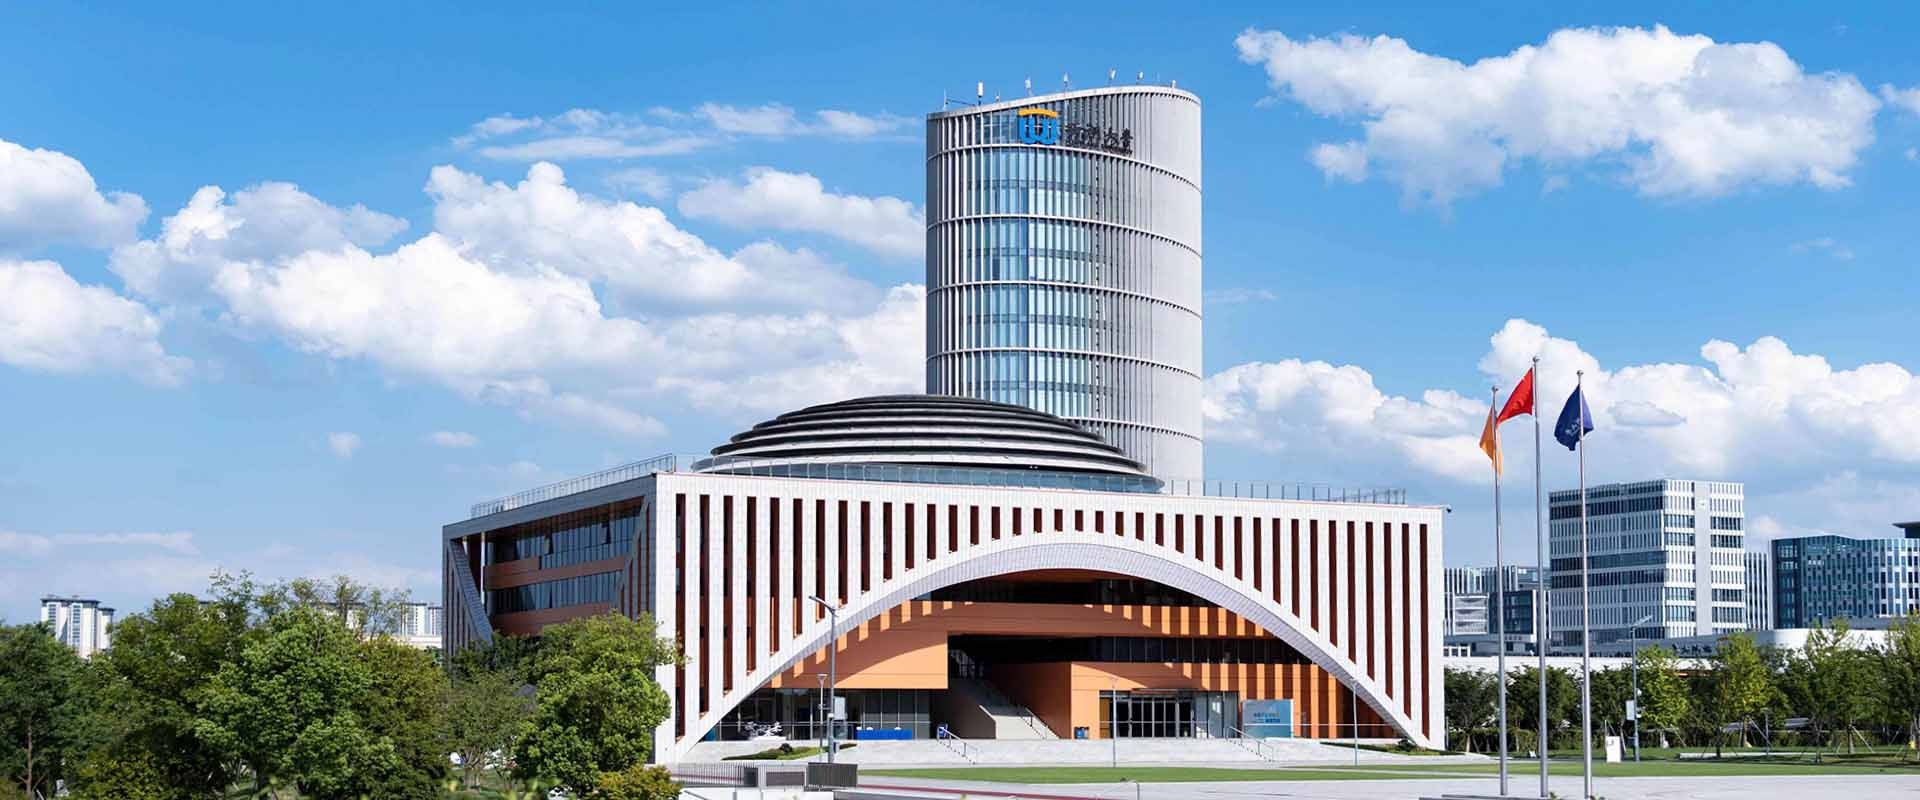
\includegraphics[width=0.8\textwidth]{./figures/westlake.jpg}
    \end{center}
            \caption{This photo was taken by Kairos at Westlake University.}
    \label{fig1}
\end{figure}
\end{lstlisting}

\begin{figure}[htbp]
    \begin{center}
        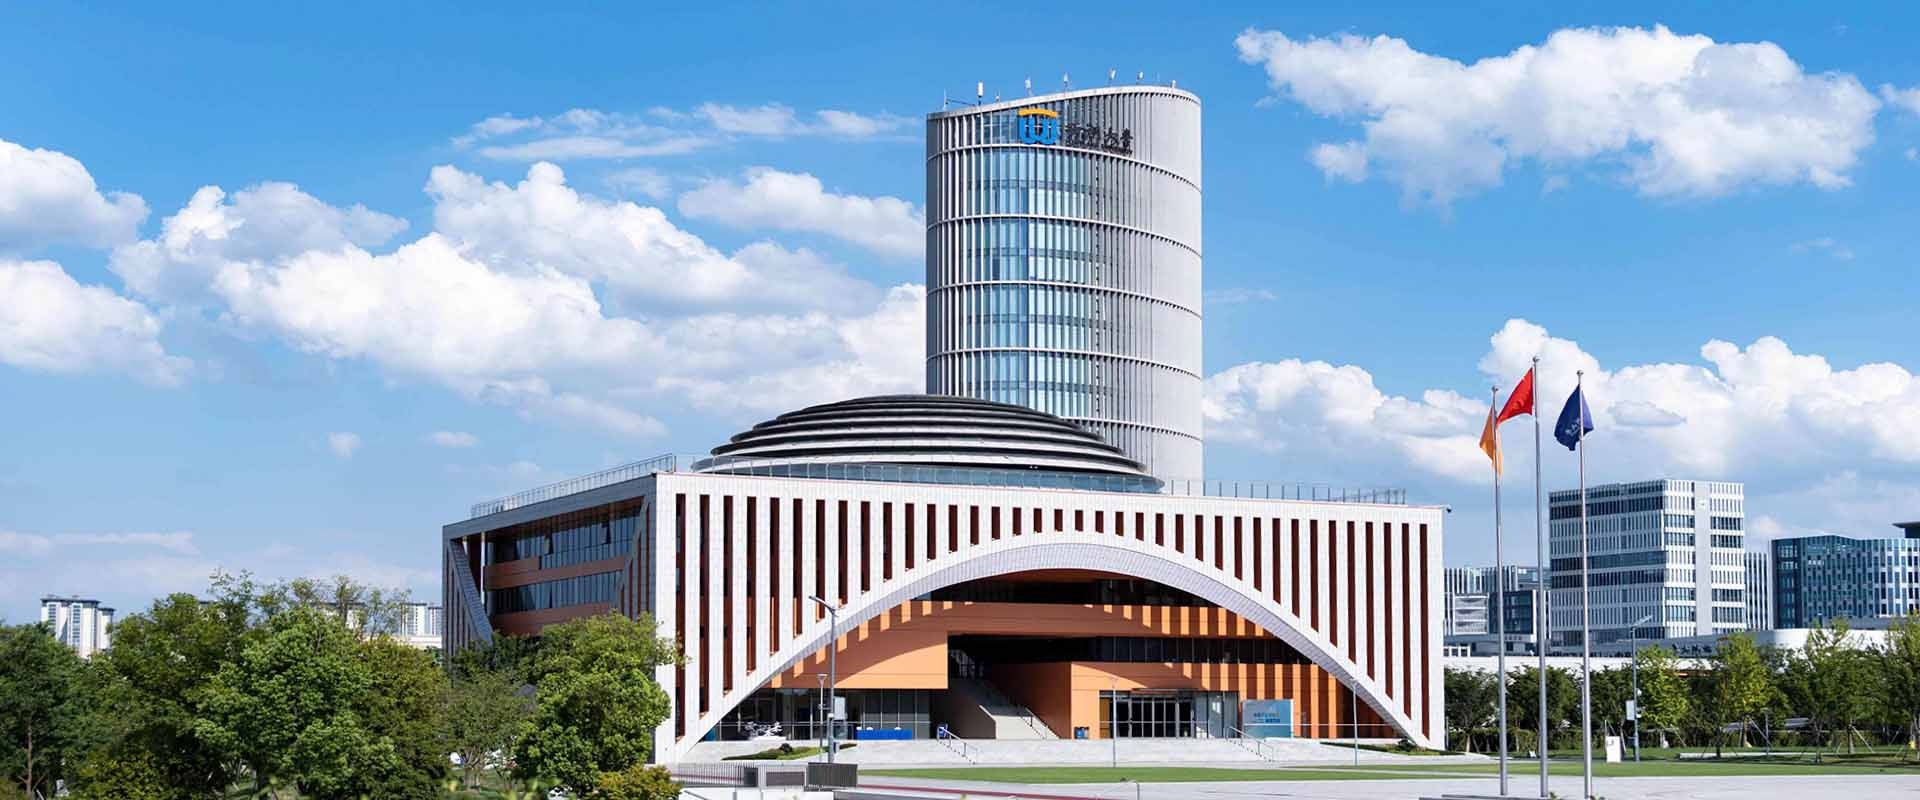
\includegraphics[width=0.8\textwidth]{./figures/westlake.jpg}
    \end{center}
            \caption{This photo was taken by Kairos at Westlake University.}
    \label{fig1}
\end{figure}

\subsection{Referencing and Hyperlinking}
\subsubsection{Linking}
To create references and hyperlinks, we could use the hyperref package.
\LaTeX\ allows us to link to figures (Fig. \ref{fig1}), tables (Table \ref{tab1}), equations (Eq. \ref{eq1}), algorithms (Algorithm \ref{alg1}), and external URLs.

\subsubsection{Bibliography}
To cite references, please use \textbackslash \texttt{cite} command followed by the citation key from .bib file. We could include those keys in .bib file to manage references for articles \cite{Article2024}, books \cite{Book2024}, websites \cite{Website2024}, and conference papers \cite{Inproceeding2024}. Here are some styles:

\begin{lstlisting}
@article{Article2024,
  author  = {Author},
  title   = {Sample Article Title},
  journal = {Journal of Samples},
  year    = {2024},
  volume  = {10},
  number  = {2},
  pages   = {123-145}
}

@book{Book2024,
  author    = {Author},
  title     = {Sample Book Title},
  publisher = {Publisher Name},
  year      = {2024},
  address   = {Publisher Address},
  edition   = {2nd}
}

@online{Website2024,
  author  = {Author},
  title   = {Sample Webpage Title},
  year    = {2021},
  url     = {http://www.example.com},
  urldate = {2024-07-22}
}

@inproceedings{Inproceeding2024,
  author       = {Author},
  title        = {Sample Conference Paper Title},
  booktitle    = {Proceedings of the Sample Conference},
  year         = {2024},
  editor       = {Editor Name},
  volume       = {1},
  series       = {Series Name},
  pages        = {45-60},
  address      = {Conference Address},
  month        = {7},
  organization = {Conference Organization}
}
\end{lstlisting}


\section{Acknowledgement}
I would like to express my sincere gratitude to all those who have supported me throughout the path of this project.


\printbibliography[title={References}]
% ------------------------------------


% ------------------------------------
% appendix
\newpage
\appendix
\section*{Appendix}
\setcounter{equation}{0}
\numberwithin{equation}{section}
\renewcommand{\theequation}{A.\arabic{equation}} 
\section{Part 1}\label{Appendix_A}
In appendix, the label of formula has been modified. Let me give you an example, Kullback-Leibler (KL) divergence $\mathbb{D}_{\mathrm{KL}}(P|| Q)$ is defined as

\begin{equation}
    \mathbb{D}_{\text{KL}}(P || Q)= \sum_{x \in \mathcal{X}} P(x)\log \left( \frac{P(x)}{Q(x)} \right) 
\end{equation}

\section{Part 2}\label{Appendix_B}
Thank you for using this template!
% ------------------------------------





